%! TeX root = ../charles/en/thesis.tex

\chapter{Background}
\label{chap:bg}

In this chapter, we briefly cover progress in obtaining useful representations
of language (\cref{sec:lm}), images (\cref{sec:imrec}), and efforts to combine
these two modalities (\cref{sec:vlm}). We then look at the extension of vision
and language models to videos (\cref{sec:vidlma}), which introduces the extra
complexity of reasoning across sequences of images, and optionally adding a
further modality, audio. Finally, we explore the literature on temporal
reasoning in language and in vision (\cref{sec:tempreason}).
%We finish the chapter with an introduction to and motivation for studying the
%task of video question answering (\cref{sec:vidqa}).

\section{Language Modeling}
\label{sec:lm}

Language modeling is the task of predicting the next word given some number of
previous words. A neural language model~\citep{bengio2003nlm} performs this by
receiving as input to a feedforward neural network a representation of previous
words in a sequence and outputting a probability distribution over possible
words. The probability of a sequence of $T$ words $w_1^T$ is thus the
combined probability of all words given their context:
$$\hat{P}(w_1^T)=\prod_{t=1}^{T}\hat{P}(w_t|w_1^{t-1})$$
The conditional probability can be approximated by using a fixed context
length, $N$, $$\hat{P}(w_t|w_1^{t-1})\approx\hat{P}(w_t|w_{t-N+1}^{t-1})$$,
greatly reducing the computational requirements for longer sequences.

\subsection{Recurrent Neural Networks}
\label{ssec:rnn}

The recurrent neural network (RNN) takes individual items from a sequence, one
at a time, and outputs a prediction based on the single unit and a hidden
state.  The hidden state is a recursive unit learnt from previous hidden
states, so that at timestep $t$, the hidden state $h_t$ is a combination of the
previous hidden state $h_{t-1}$ and the current input $x_t$. The hidden state
is therefore a representation of the entire input sequence up to time $t$. This
avoids the problem faced by feedforward neural language models of only
representing a limited context window of size $N$. In theory, an RNN can
represent an unlimited context.

In practice, RNNs struggle to encode long-distance dependencies well, with the
information encoded in hidden states being biased towards more recent items of
the input, and struggling from the vanishing gradient problem, whereby repeated
matrix multiplications for backpropagation through time drive the gradient to
zero. The main extension to the RNN, the long short-term memory (LSTM)
network~\citep{hochreiter1997lstm}, modifies the architecture of the recurrent
unit to include three gates: the forget gate, the add gate, and the output
gate. Combined, these three gates keep the context vector, the previous hidden
state, simple by removing information considered no longer useful, add useful
information from the current input, and output information considered useful
for the current hidden state.

RNNs are often used in sequence-to-sequence, or encoder-decoder, set-ups, in
which the input sequence is processed by the encoder section, creating a
context vector which is a representation of the entire input sequence. This is
then fed as the initial hidden state of a decoder network to generate the
output. The benefit of this is that the output size is not related to the input
size. For tasks such as machine translation, image captioning, or open-ended
question answering, the ability to generate an answer is critical.

The bottleneck problem is alleviated slightly by the attention
mechanism~\citep{bahdanau2015attention}, where an additional context vector is
used by the decoder to dynamically attend to different hidden states of the
encoder based on the current input token in the decoder. This context vector is
created by a weighted sum of encoder hidden states, recomputed at each timestep
during decoding. Attention with RNNs improved the state of the art in machine
translation, particularly on sentences with longer input. It has also been used
in vision and language models to attend to key parts of the image vector
for visual question answering~\citep{yang2016san}.


\subsection{Transformer}
\label{ssec:transformer}

\citet{vaswani2017attention} introduced the Transformer architecture for
sequence tasks, replacing the recurrent nature of the RNN and its variants with
multi-head self-attention. This allows for parallel computation since
computation at each timestep is independent of all others, greatly increasing
the ability to train on larger and larger data and model sizes. Self-attention
assigns attention scores to each item of the input sequence itself, regardless
of input size, to compute a representation of the sequence. The Transformer
uses stacked layers of self-attention to capture the many ways that an input
sequence can relate to itself. Each self-attention head can learn to encode
different relationships between sequence tokens, and these heads are combined
and linearly projected into the original dimensionality.
\citet{vaswani2017attention} use attention between the encoder and decoder, so
each position in the decoder can attend to all items of the input sequence, and
further use self-attention in both the encoder and decoder. In the decoder, a
modification is made to prevent knowledge of future information being
generated, masking out all values in the input that correspond to future input
connections. Finally, positional encodings are included for each token to keep
some notion of sequence order that would otherwise be lost from the RNN
architecture. The Transformer achieved state of the art performance on machine
translation, and has since been used as the de facto architecture for many
sequence tasks, in both language and vision.

\subsection{Masked Language Modeling}
\label{ssec:mlm}

BERT~\citep{devlin2019bert} uses only the encoder layers of the Transformer to
create strong representations of an input sequence. Since it is trivial to
predict the next token in a sequence when provided with the entire context,
BERT, and its descendants such as RoBERTa~\citep{liu2020roberta}, train on a
masked language modeling objective on unlabeled data, where the task is to mask
some percentage of the input tokens at random, and then predict those masked
tokens.

These representations on their own are not especially useful, but once trained,
they provide a great starting point for finetuning to a specific task, where
there may not otherwise be enough data to learn these rich representations of
language. Downstream tasks can include question answering, natural language
inference, or sentence classification. Pre-training then finetuning has become
a common paradigm due to the relative low cost of finetuning once a large model
has been pre-trained. BERT achieved state of the art on eleven NLP tasks, all
of which were finetuned in less than an hour on a TPU. BERT has successfully
been adapted to vision and language models, as we will discuss in
\cref{sec:vlm}.


\section{Image Recognition}
\label{sec:imrec}

A key part of video and language models is learning representations of frames
in sequence, which involves the classical tasks of object detection, image
segmentation, and image classification. Much like in NLP, the standard approach
is to pre-train on large image datasets and finetune to a specific desired
task. Convolutional neural
networks~\citep{lecun1989lenet,krizhevsky2012alexnet,he2016resnet} use
convolution kernels, pooling, and optionally batch normalisation, dense or
residual layers to create representations of image features.
AlexNet~\citep{krizhevsky2012alexnet} uses a multi-layer convolutional neural
network (CNN) to classify images from ImageNet~\citep{deng2009imagenet}, a
dataset of over 15 million images from around 22,000 categories, and was the
first to show the scaling power of large datasets and model sizes for producing
strong image features. 

There have been attempts to combine CNN architectures with self-attention
mechanisms. This may provide more scope for non-local computation which may be
required on tasks such as object detection with large objects. However, due to
the quadratic cost of self-attention in the number of pixels, naive
implementations are infeasible, and approximations struggle to scale
efficiently~\citep{carion2020detr}. The Vision
Transformer~\citep{dosovitskiy2021vit} does away with the CNN for image
recognition, and uses an adapted version of the Transformer for greater
scalability.


\subsection{Vision Transformer}
\label{ssec:vit}

\citet{dosovitskiy2021vit} introduced the Vision Transformer (ViT), which takes
the impressive performance of the Transformer architecture on sequence tasks
and applies it to image tasks. The authors represent an image as a sequence of
patches of an image, with an extra patch embedding added alongside the
positional embedding of the Transformer \citep{vaswani2017attention} to maintain
the 2-dimensional information of an image when projected into a linear
sequence. The model is shown in \cref{fig:vit}. The Vision Transformer matched
or exceeded state of the art on many image classification datasets, while being
trained for comparatively less time.

\begin{figure}[tp]
	\centering
	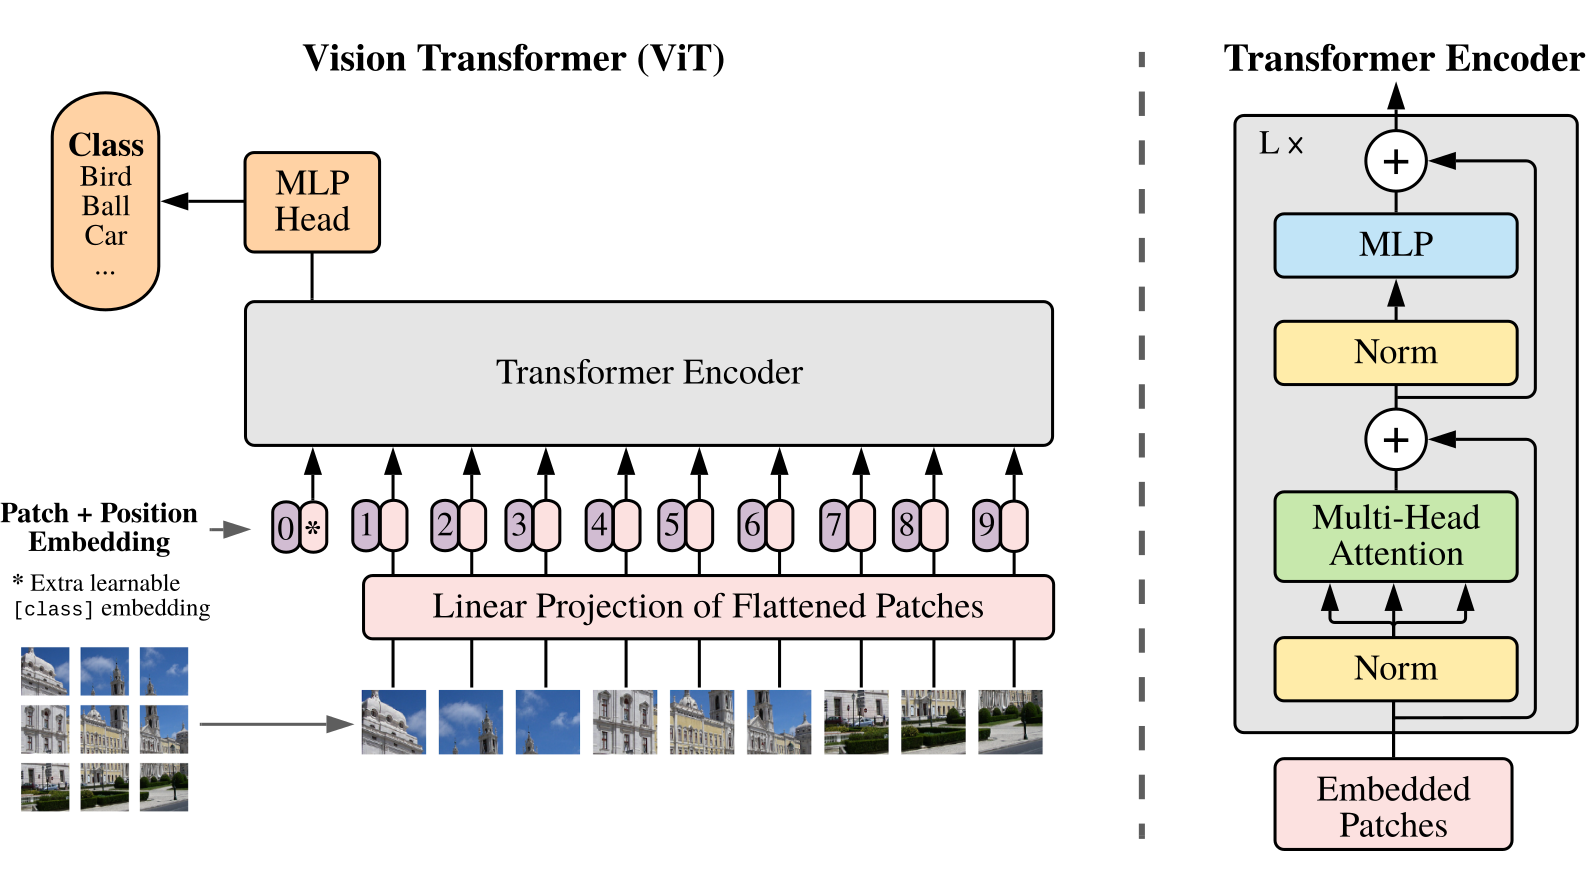
\includegraphics[width=0.8\textwidth]{vit.png}
	\caption{The Vision Transformer splits an image into patches, embeds them,
		and feeds them into a Transformer encoder. Classification is learned
		via an MLP head following the encoder. Figure reproduced
		from~\citet{dosovitskiy2021vit}}
	\label{fig:vit}
\end{figure}


\subsection{CLIP}
\label{ssec:clip}

\citet{radford2021clip} introduced CLIP (Contrastive Language-Image
Pre-training), which uses the Info-NCE loss~\citep{oord2019infonce} to jointly
learn relationships between encodings of text captions and extracted feature
representations of associated images. The Info-NCE loss trains a multimodal
embedding space to maximise the cosine similarity of matching pairs of captions
and images, while minimising the cosine similarity of non-matching pairs in the
batch. The approach is shown in \cref{fig:clip}. A key part of this approach is
using a very large batch, so that there are many incorrect pairings to learn
from. \citet{radford2021clip} use a batch size of 32768. The text encoder is a
Transformer~\citep{vaswani2017attention}, and their best model uses a Vision
Transformer~\citep{dosovitskiy2021vit} as the image encoder.

The model enables zero-shot transfer to many downstream computer vision
classification tasks by predicting the most probable (image, text) pair when
given an image and a set of text prompts with each class embedded in the prompt
achieving performance comparable to or surpassing the previous state of the art
by finetuned models. The representations learned by the contrastive
pre-training objective have wide applicability to a range of VLM and Video
Language Models, particularly as frozen features from which to add smaller
modules on top for adapting to vision and language
tasks~\citep{alayrac2022flamingo,lin2022evl,luo2022clip4clip}. We discuss some
of these models in \cref{sec:vidlmb}, and consider the limitations and possible
expansions of the contrastive pre-training method in \cref{sec:contrastive}.

\begin{figure}[tp]
	\centering
	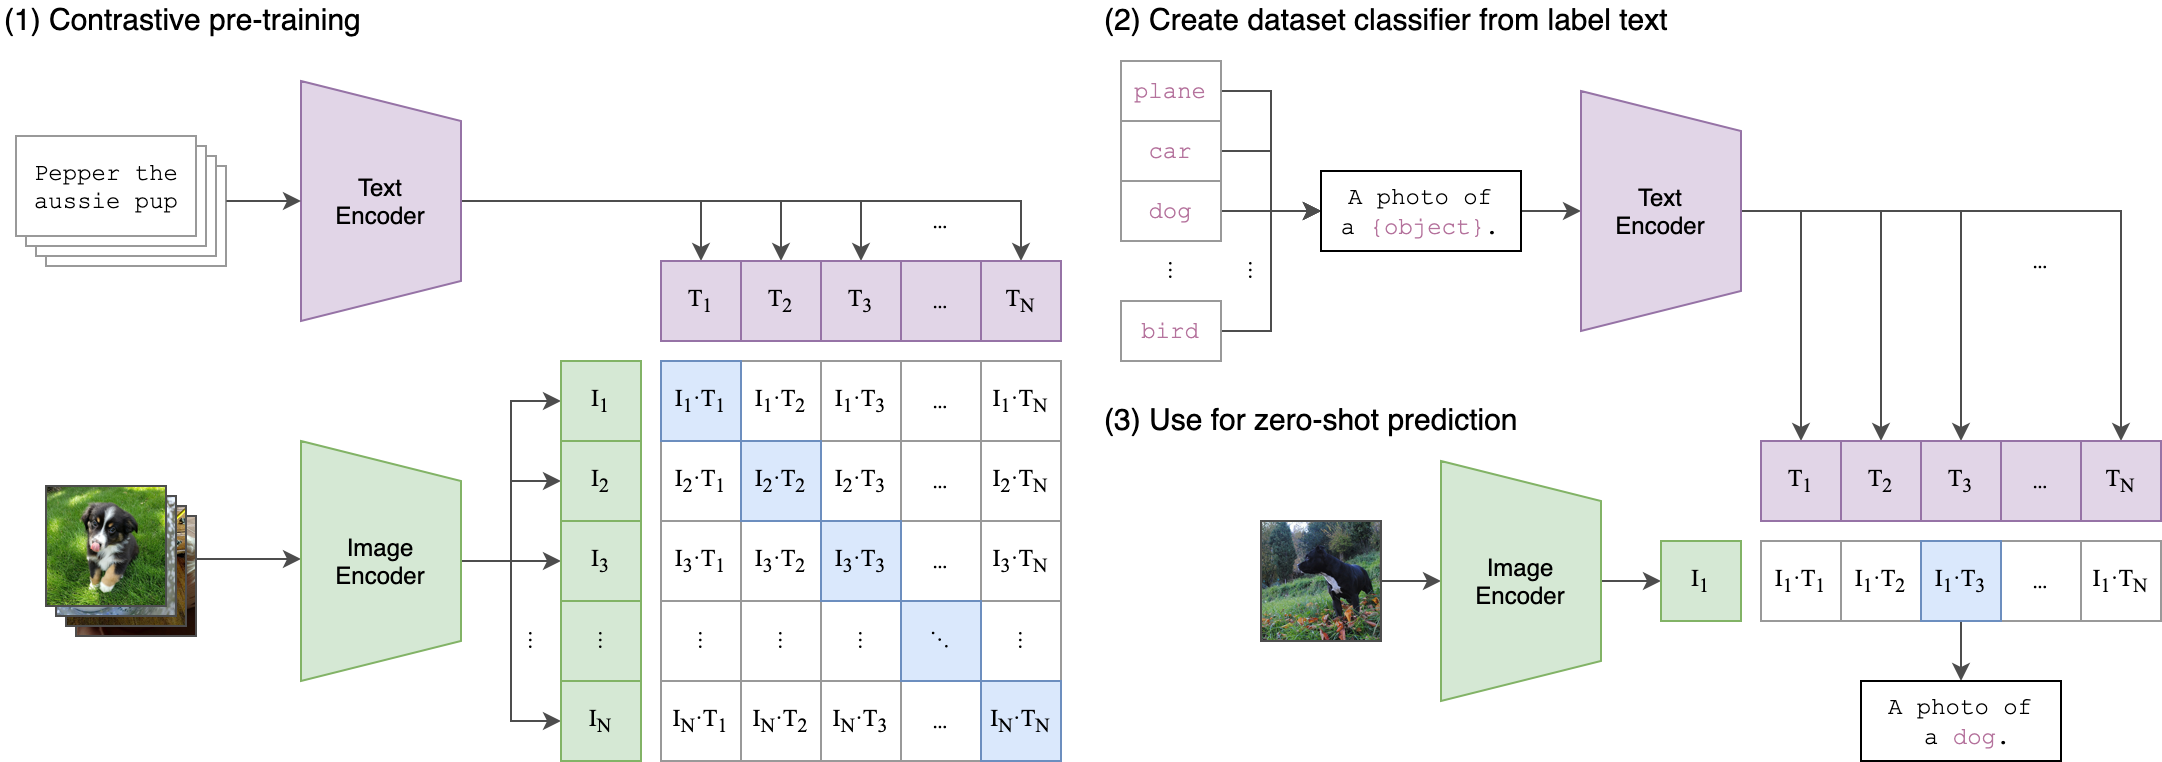
\includegraphics[width=\textwidth]{CLIP.png}
	\caption{CLIP. From~\citet{radford2021clip}}
	\label{fig:clip}
\end{figure}


\section{Vision and Language Models}
\label{sec:vlm}

One criticism of language models is that the representations learned by
training a model to predict the next word fail to learn any kind of
meaning~\citep{bender2020climbing} without reference to the real world. Models
trained in this way learn connections between surface forms, but no grounded
meaning between the form and intent portrayed through the form. A way to create
grounded representations may be to combine the two modalities of language and
vision through multimodal embeddings. A key challenge in recent years has been
to find suitable methods for creating these shared representations.

Following the strong performance in NLP of BERT~\citep{devlin2019bert},
\citet{li2019visualbert} extend BERT to include visual features extracted from a
CNN as well as text tokens as input to a Transformer encoder, implicitly
discovering a joint representation between the two modalities. The authors use
the self-attention mechanism to align elements of the input text and regions in
the input image, and pre-train on two visually-grounded language model
objectives. The authors finetune and evaluate on a range of vision and language
applications, including visual question answering (see below).

%\cite{lu2019vilbert}

Other approaches take frozen encodings of image, text, or both, and learn a
shared embedding space on top of this (e.g. BLIP-2 \citep{li2023blip2})

%Many approaches, joint training with concatenated image and text features into
%BERT (VisualBERT), learning both image and text features concurrently.


\subsection{Visual Question Answering}
\label{ssec:vqa}

Visual question answering is the task of answering questions given text and an
image. There are a wide range of datasets (name some). A challenge in creating
datasets is to ensure that there are few statistical biases or shortcuts in the
answer distribution that a model can exploit without a true understanding of
the scene. For example, models trained on the VQA dataset~\citep{antol2015vqa}
were found to make predictions based on overly strong language priors without
considering the associated image~\citep{zhang2016yin} (a green banana may trip
up a model) and failed to show complete question understanding, settling on an
answer before receiving the full question ~\citep{agrawal2016analyzing}.
Questions generally required little reasoning or compositionality, with many
answers achievable solely by object recognition~\citep{hudson2019gqa}. The GQA
dataset~\citep{hudson2019gqa} is one dataset that aims to limit these issues
by generating questions with linguistic diversity and a large vocabulary, and
balancing the answer distribution through sampling. 

Visual question answering has also been extended to question answering over
videos. On top of scene understanding, video question answering requires event
understanding to understand causal and temporal relationships within the
context of the video. A particular challenge in developing models for this task
is combining and aligning the modalities of text, vision, and audio as well.
Numerous datasets have been proposed for this task,
e.g.~\citet{xu2016msr-vtt,wu2021star,xiao2021nextqa,lei2020tvqaplus}. We discuss
two, STAR~\citep{wu2021star} and NExT-QA~\citep{xiao2021nextqa}, in
\cref{chap:dataset}.


\section{Video Language Models}
\label{sec:vidlma}

%Models which solve video tasks. How to choose frames, methods for learning
%temporal aspect, modeling sequences of images
Much as the task of visual question answering has been extended to the domain
of video, so too have models been created for video language tasks. Video
language models are models used to solve problems related to video
understanding tasks. This introduces the added complexity of temporal modeling
to understand relationships between successive frames in the video, as well as
the possibility of modeling audio where the data allows it. There are two main
ways of solving these tasks. The first is to use pretrained vision and language
models we saw previously to the new domain without any specific training or
finetuning on a video dataset.  Alternatively, we can train on a video dataset,
either from scratch, or finetuning from a pretrained vision and language model.
This section explores both methods.

\subsection{Adapted from Vision and Language Models}
\label{ssec:adaptvlm}

Pre-trained generative language models have shown strong capabilities for
in-context learning~\citep{brown2020gpt3}. In-context learning provides a number
of examples of a task (for few-shot learning -- zero-shot learning provides only
a task description) as the start of a prompt to a language model, where a
typical example contains the context of the task and its desired completion.
The language model must then provide the correct completion when presented with
just the example context. This idea, and extensions, have been shown to be
effective for a wide range of tasks, particularly those which require advanced
reasoning~\citep{wei2022cot,kojima2022step}.

By providing generative language models with access to image features in its
prompt, it is possible to leverage pre-trained language models for video tasks.
\citet{wang2022vidil} use a vision and language model to label objects, events
and attributes, as well as captions, for each sampled frame in a video. These
features are then composed in a template for few-shot learning of video tasks.
Temporal relationships between frames are modeled in the template using textual
indicators (`first', `then', `finally'). Crucially, no finetuning of language
or vision and language models is performed, so high quality pretrained models
can be plugged in and changed easily. This process is highly dependent on
strong visual feature extraction, meaning that key low-level features may be
lost if the vision models are not strong enough. Concurrent work
by~\citet{zeng2023socratic} finds that using stronger vision and language
models correlates with better performance when combining VLMs and LMs in a
zero-shot manner for egocentric perception. Finally, the added latency costs of
having separate models for visual tokenisation, frame captioning, and language
generation may make the overall system inadequate for practical use.

\citet{portilloquintero2021clipvidret} use CLIP features with an aggregation
function across frames to adapt to the video domain for retrieval tasks. The best
aggregation function tested was to simply average frame-level features, which
beat previous best recall@1 scores on the MSR-VTT~\citep{xu2016msr-vtt} dataset.
The authors found that using a single frame from around one second in to the
video as the aggregation function gives significantly worse recall performance
than other aggregation functions which take into account multiple frames.

By contrast, \citet{huang2018videotemporal} found that temporal understanding
plays just a small role in multiple video datasets. On two action recognition
datasets, the impact of motion accounts for just 6 percentage points of 79\%
accuracy on UCF101~\citep{soomro2012ucf101}, and 5 points of 47\% accuracy on
Kinetics~\citep{carreira2018kinetics600}, and 40\% and 35\% of classes do not
require any temporal understanding for the two datasets respectively.
\citet{buch2022revisiting} extend this finding for video language tasks, with
single frame understanding performing strongly compared to state of the art
models, ``even in settings intended for complex multi-frame event
understanding''. The key distinction between these works
and~\citet{portilloquintero2021clipvidret} is that the model selects a highly
informative frame based on its task. \citet{buch2022revisiting} propose that
their design, the atemporal probe (ATP), should be used to design better
datasets that better test efficacy of a benchmark for causal and temporal
understanding. They find a subset of NExT-QA~\citep{xiao2021nextqa} questions
that ``truly necessitate video-level understanding compared with the original
dataset''. We test on both NExT-QA and this subset, denoted
ATP\textsubscript{hard}, in our experiments.

%Either train with explicit temporal tokens (e.g.~\citet{lin2022evl} with temporal convolution and cross-frame attention, \citet{lei2021clipbert} with temporal fusion and sequential frames and word embeddings) or use language to steer temporal modality \citep{wang2022vidil,zeng2023socratic}.


%\citet{zeng2023socratic} -- Similar idea to VidIL, but zero-shot composition


\subsection{Training on Videos}
\label{ssec:vidtrain}

%Models which take into account temporal nature and train/finetune on video datasets

Since one of the questions we are interested in is how contrastive training
affects the temporal reasoning ability of video language models, this section
mainly explores models trained with a contrastive objective. We note, however,
that other models~\citep{lei2021clipbert} (and others!!) have achieved
comparable downstream performance when trained with other objectives (masked
language modeling, image-text matching, cross-modal attention).

The obvious approach for training video models is to train on videos.
\citet{luo2022clip4clip} extend image and language models to video retrieval in
a simple way by mapping sequences of image representations learned from CLIP
into a fixed video representation, and computing similarity between the CLIP
text encoding and the learned video encoding. They find that training on a
medium-sized video dataset starting from the CLIP encodings improves zero-shot
and finetuning results on multiple downstream datasets, and that attempts to
model the temporal dependency between frames (using 3D linear projections for
video features, and using similarity measurements that model sequentiality for
the video and text similarity measure) from the base CLIP model trained only on
image and text pairs do not produce better results on video tasks.

\citet{bain2021frozen} train separate visual encoder for image and video and text encoder for captions

\cite{xu2021videoclip}


%\citet{lin2022evl} -- train video recognition models from frozen CLIP features
\citet{lei2021clipbert} -- temporal fusion and sequential frames and word embeddings

\citet{alayrac2022flamingo} -- train on combination of image-text, video-text pairs datasets. Vision encoder is CLIP. Temporal embeddings are combined with visual features and processed via a resampling module, allowing for a variable number of frames to produce a fixed size visual output, which is advantageous for longer videos.

\section{Temporal Reasoning}
\label{sec:tempreason}


\noindent\textbf{In Video.}\hspace{0.2cm}
Most computer vision has studied how to model concepts and relationships
between them in the world, e.g. through object detection and segmentation in
images. To go one step further into the video domain, we need to study how to
model event knowledge. That is, how do we model recurring and meaningful
patterns and sequences of behaviour? A model must understand activities and
their components, as well as the temporal ordering of these activities to find
causal dynamics between them~\citep{elman2019event}. New datasets and models
have been proposed in recent years that aim to find computational models
capable of this event knowledge through temporal reasoning. 

As discussed in~\cref{ssec:adaptvlm}, some models can still perform well on
video datasets with just a single frame given to the model. This suggests a
requirement for more challenging datasets and tasks to learn temporal ordering
of events. \citet{grauman2022ego4d} create Ego4D, a dataset of over 3000 hours
of egocentric (first-person) video, with several associated tasks requiring
understanding of how objects change state over time, remembering temporal
windows for objects appearing in scenes, and prediction of future actions in
videos, requiring causal understanding of actions and events. For example, a
cooking video may predict the subsequent steps to making a pizza when presented
with the first steps of rolling and kneading dough. The authors identify
normalised pointwise mutual information as a means to inform the temporal
structure of sequences of actions over time, with certain action sequences
favoured over others. Learning this structure of action pairs is key to a
model's performance on these tasks.\\

\noindent\textbf{In Language.}\hspace{0.2cm}
There is a long history of studying temporal expressions in linguistics.
~\citet{moens1988temporal} claim that \textit{when}-clauses ``establish a
temporal focus'' between two events, contingent on e.g. a causal link, as in
the unnatural use of \textit{when} in ``*When my car broke down, the sun set.''
Any representation looking to model temporal descriptions must therefore, for
\textit{when}-clauses and similar phenomena, model contingency, rather than
just temporality.

\citet{allen1983interval} suggests a model of temporal reasoning based on
intervals and relations among them. Given two events, the temporal relations
between them can be expressed in many ways based on the time intervals of the
events occurring. We explore the use of this temporal representation further
in~\cref{sec:data}. \citet{zhou2021tracie} propose a dataset for natural
language inference of temporal relations for before and after relations. They
find that current models struggled to predict temporal relationships between
explicit and implicit events, and that a neuro-symbolic method improved 
reasoning ability by estimating event durations to infer implicit end times.\\

%Traditional methods
%\cite{bruce1972temporalqa}
%\cite{pustejovsky2003timeml}

%Pre-trained LLMs struggle on temporal reasoning, need finetuning.~\citet{vashishtha2020temporal}

\noindent\textbf{Probing video datasets.}\hspace{0.2cm}
\citet{sevilla-lara2021temporal} create a perceptual test to discover action
classes in videos that require temporal information to identify. The authors
shuffle frames in time from action classification datasets, and present human
annotators with the shuffled or control videos, where there is no shuffling.
Action classes are then identified by the largest average performance
degradation of action classification between the two groups. They train video
models on a temporal and static dataset, the 50 classes where human accuracy
decreases most and least respectively, and find that training on the temporal
dataset produces features that are more sensitive to temporal ordering, and
therefore are stronger temporal features.
We extend this finding and explore the performance of various models with
frames shuffled on video question answering datasets in \cref{chap:probe}, and
develop a novel method for training video language models on a temporal-aware
dataset in \cref{chap:setup}.

%\section{Video Question Answering}
%\label{sec:vidqa}
%
%\subsection{STAR Dataset}
%\label{ssec:star}
%
%We primarily focus on this due to its focus on sequential questions that evaluate model performance on temporal reasoning
%
%\subsection{Merlot Reserve}
%\label{ssec:mreserve}
%
%We examine a specific video language model, Merlot Reserve \citep{zellers2022mreserve}, that performs strongly on STAR.
